\documentclass{article}
\usepackage{tikz}
\usepackage[margin=1in]{geometry}
\usetikzlibrary{positioning}
\usetikzlibrary{shapes, arrows}
\begin{document}


\centerline{\sc \large Operating Systems Writeup}
\vspace{.5pc}

\begin{flushleft}
\textbf{Name:} Joshua Abraham
\vspace{.5pc}

\textbf{Date:} 2 November 2017
\vspace{.5pc}

\textbf{Current Module:} Operating Systems
\vspace{.5pc}

\textbf{Project Name:} "Relay"
\vspace{.5pc}

\textbf{Project Goals:}
\vspace{.5pc}
\end{flushleft}

The relay project aims to create two programs that communicate via Interprocess 
Communication.  This IPC will be one-way, sending input from a
"\textbf{dispatcher}" program 
that takes input from standard input to a "\textbf {listener}" program which 
then prints text sent to the first program.
\vspace{.5pc}

\begin{flushleft}
\textbf{Considerations:}
\vspace{.5pc}
\end{flushleft}

\begin{itemize}
	\item[$\bullet$] \textbf{Dispatcher} must take text from stdin and exit when
	it receives an EOF.
	\item[$\bullet$] \textbf{Listener} should exit if the listener is closed or
	not running.
	\item[$\bullet$] Multiple \textbf{listeners} should be able to run 
	simultaneously from different users/directories.
\end{itemize}
\vspace{.5pc}

\begin{flushleft}
\textbf{Initial Design:}
\vspace{.5pc}
\end{flushleft}

The project is composed of the following files:
\begin{itemize}
	\item [$\cdot$] \textit{Makefile}: The main makefile for the project.
	\item [$\cdot$] \textit{dispatcher.c}: The source code for the 
	\textbf{dispacher}.
	\item [$\cdot$] \textit{listener.c}: The source code for the 
	\textbf{listener}.
	\item [$\cdot$] \textit{relay.c}: The source code with a helper function
	used by both programs.
	\item [$\cdot$] \textit{relay.h}: The header file for the project.
\end{itemize}
\vspace{2mm}

\begin{flushleft}
\textbf{Data Flow:}
\vspace{.5pc}
\end{flushleft}

The data flow from \textbf{dispatcher} to \textbf{listener} is as follows:

\begin{center}
\begin{equation}
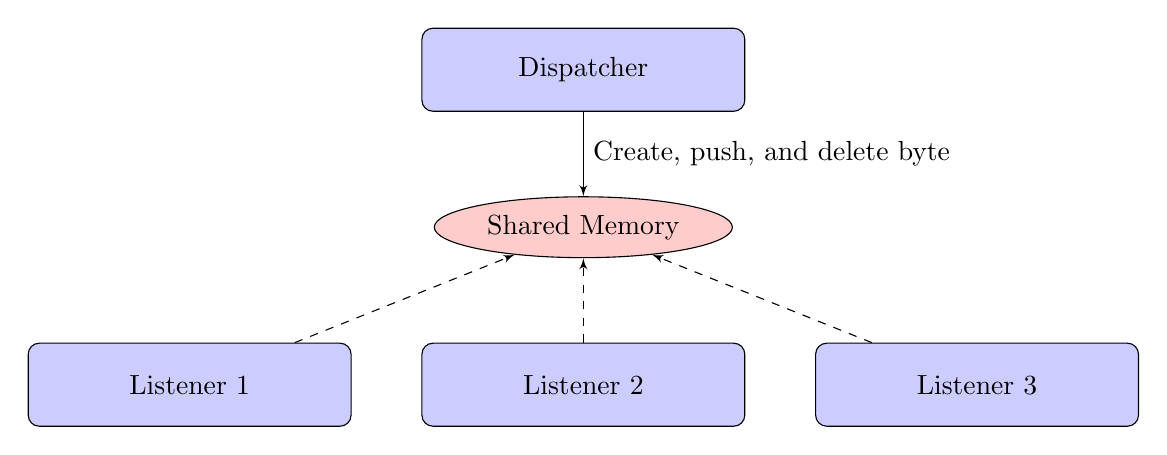
\begin{tikzpicture}[node distance = 2cm, auto]
    text width=4.5em, text badly centered, inner sep=0pt]
    \tikzstyle{block} = [rectangle, draw, fill=blue!20, 
    text width=11em, text centered, rounded corners, minimum height=3em]
    \tikzstyle{line} = [draw, -latex']
    \tikzstyle{cloud} = [draw, ellipse,fill=red!20, minimum height=2em]
    \node [block] (dispatcher) {Dispatcher};
    \node [cloud, below of=dispatcher] (memory) {Shared Memory};
    \node [block, below of=memory] (listen2) {Listener 2};
    \node [block, right of=listen2, node distance = 5cm] (listen3) {Listener 3};
    \node [block, left of=listen2, node distance = 5cm] (listen1) {Listener 1};
    \path [line] (dispatcher) -- (memory) node [midway] {Create, push, and delete byte};
    \path [line, dashed] (listen1) -- (memory);
    \path [line, dashed] (listen2) -- (memory);
    \path [line, dashed] (listen3) -- (memory);
\end{tikzpicture}
\end{equation}
\end{center}

My project operates character by character, byte by byte on input from the 
user. Input is given to the running dispatcher which has changed the terminal 
settings to non-cannonical mode in order to get data unbuffered. Each 
character is copied to the one byte shared memory segment then the dispatcher
sleeps for 5000 nanoseconds. Then, the shared memory segment is set to NUL. 
Before the shared memory is set to NUL, the listener prints the data and then 
sleeps for 5000 nanoseconds. This loop is performed until the user gives a 
control-D to the dispatcher. In order to prevent a control-C from prematurely
ending the dispatcher (which would result in the shared memory segment not
being deleted), a tiny SIGINT handler is used at the beginning of the program.
The listeners test for the existence of the shared memory segment and if it 
does not exist, the listener exits cleanly. Once the user sends a control-D to
the dispatcher, the dispatcher sets the shared memory to EOT which is the 
magical number that closes the listeners. 
\vspace{.5pc}

\begin{flushleft}
\textbf{Communications Protocol:}
\vspace{.5pc}
\end{flushleft}

The dispatcher and listener performed IPC via System V shared memory. This 
communication was one-way and used exactly one byte of memory.  
\vspace{.5pc}

\begin{flushleft}
\textbf{Potential Pitfalls:}
\vspace{.5pc}
\end{flushleft}

\begin{itemize}
	\item[$\bullet$] Listeners re-printing data in shared memory before it is 
	deleted.
	\item[$\bullet$] Listeners closing when user gives a control-D to the 
	dispatcher.
	\item[$\bullet$] Dispatcher not prematurely closing before sending EOT to
	listeners. 
\end{itemize}
\vspace{.5pc}

\begin{flushleft}
\textbf{Test Plan:}
\vspace{.5pc}
\end{flushleft}

\textit{User Tests:}
\begin{itemize}
	\item[$\cdot$] Performed test specified in the project supplement manual.
	\item[$\cdot$] Sent dispatcher a control-C in the middle of execution.
	\item[$\cdot$] Checked system IPC mechanisms via the "ipcs" command to 
	ensure that all shared memory is deleted after successful execution.
\end{itemize}

\textit{Test Cases:}
\begin{itemize}
	\item[$\cdot$] Tested SIGINT handler and shared memory deletion.
	\end{itemize}
\vspace{.5pc}

\begin{flushleft}
\textbf{Conclusion:}
\vspace{.5pc}
\end{flushleft}

The relay project was a learning experience for me. I learned about the
various IPC mechanisms that UNIX provides such as message queues, semaphores,
shared memory, etc. I decided to utilize shared memory after reading the 
textbook and deciding that this method was best for one way, multicast 
communication. I initially planned on using semaphores for the dispatcher to 
keep track of all listeners, however, I decided that it added unneeded 
complexity and simply used the EOT character to terminate the listeners. 
Throughout the development of the project, I chose to prioritize efficiency
and simplicity in order to produce a fast, accurate program. This is why I 
chose to operate character by character and to only use one byte of shared
memory. I am very happy with the outcome. The only possible change for the 
future would be to use a faster mechanism for getting data from the shared 
memory. 

\end{document}